\chapter{Results and Discussion}
\label{chapter:Results and Discussion}



% Here starts the thesis with an introduction. Please use nice latex and bibtex entries \cite{latex}. Do not spend time on formating your thesis, but on its content. 
 
\section{Results and Discussion}
In this chapter, we evaluate the proposed algorithm using real data acquire using 
the camera rig system shown in \ref{ fig:rigsetup} and compare result with different 
approaches \todo{ define approaches}



There is no need for a latex introduction since there is plenty of literature out there.
% \begin{figure}%
% \centering
% \subfloat[][]{res/ram/3/im0218.jpg}%
% \qquad
% \subfloat[][]{res/ram/3/im0218.jpg}
% \caption{Here are the first two figures of a continued figure.}%
% \label{fig:cont}%
% \end{figure}


\begin{figure}
\begin{adjustwidth}{-1in}{-1in} 
\centering     %%% not \center
\subfigure[Figure A]{\label{fig:a}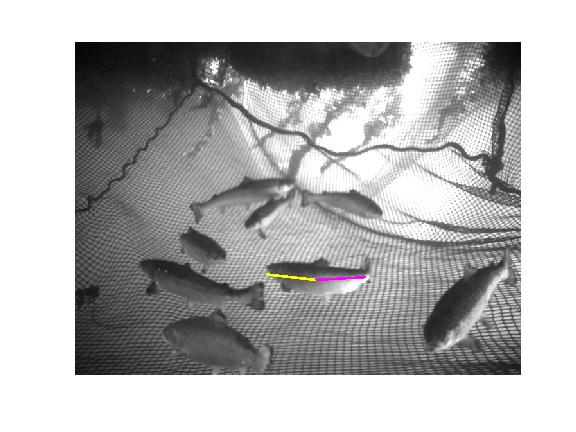
\includegraphics[width=50mm]{res/ram/3/im0218.jpg}}
\subfigure[Figure B]{\label{fig:b}\includegraphics[width=50mm]{res/ram/3/im0219.jpg}}
\subfigure[Figure C]{\label{fig:c}\includegraphics[width=50mm]{res/ram/3/im0220.jpg}}
\subfigure[Figure D]{\label{fig:d}\includegraphics[width=50mm]{res/ram/3/im0221.jpg}} \\
\subfigure[Figure A]{\label{fig:a}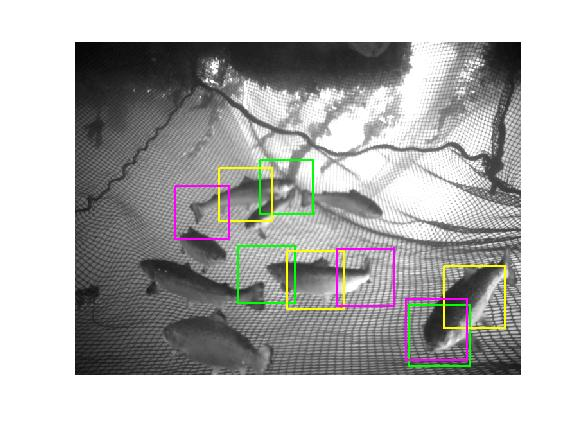
\includegraphics[width=50mm]{res/ram/3/im0218_m.jpg}}
\subfigure[Figure B]{\label{fig:b}\includegraphics[width=50mm]{res/ram/3/im0219_m.jpg}}
\subfigure[Figure C]{\label{fig:c}\includegraphics[width=50mm]{res/ram/3/im0220_m.jpg}}
\subfigure[Figure D]{\label{fig:d}\includegraphics[width=50mm]{res/ram/3/im0221_m.jpg}}
\caption{my caption}
\end{adjustwidth}
\end{figure}


\begin{figure}
\begin{adjustwidth}{-1in}{-1in} 
\centering     %%% not \center
\subfigure[Figure A]{\label{fig:a}\includegraphics[width=50mm]{res/ram/5/im0219.jpg}}
\subfigure[Figure B]{\label{fig:b}\includegraphics[width=50mm]{res/ram/5/im0220.jpg}}
\subfigure[Figure C]{\label{fig:c}\includegraphics[width=50mm]{res/ram/5/im0221.jpg}}
\subfigure[Figure D]{\label{fig:d}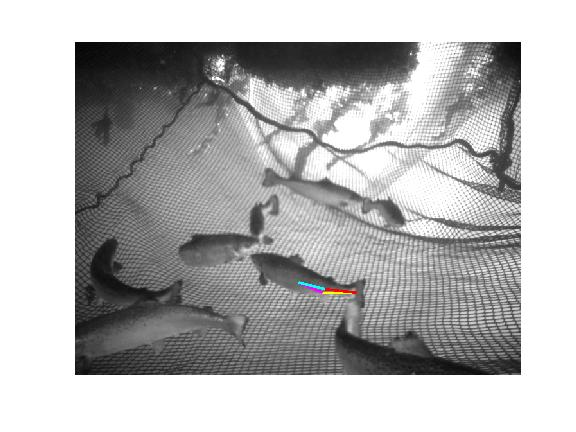
\includegraphics[width=50mm]{res/ram/5/im0222.jpg}} \\
\subfigure[Figure A]{\label{fig:a}\includegraphics[width=50mm]{res/ram/5/im0219_m.jpg}}
\subfigure[Figure B]{\label{fig:b}\includegraphics[width=50mm]{res/ram/5/im0220_m.jpg}}
\subfigure[Figure C]{\label{fig:c}\includegraphics[width=50mm]{res/ram/5/im0221_m.jpg}}
\subfigure[Figure D]{\label{fig:d}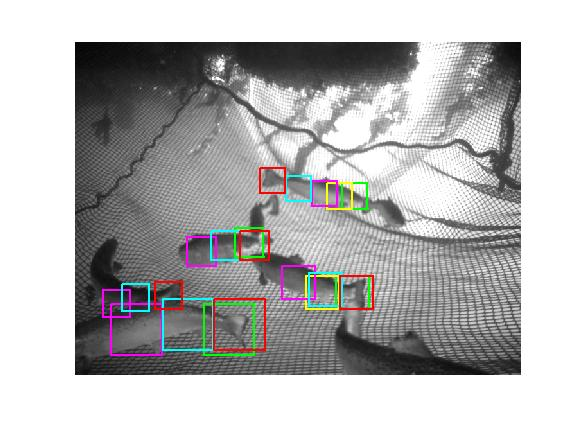
\includegraphics[width=50mm]{res/ram/5/im0222_m.jpg}}
\caption{my caption}
\end{adjustwidth}
\end{figure}

\section{Conclusion}
There is no need for a latex introduction since there is plenty of literature out there.


% \section{Next Section}
% There is no need for a latex introduction since there is plenty of literature out there.
